\documentclass[10pt,a4paper]{article}
\usepackage{fontspec}
\setmainfont{Arial}
\usepackage[spanish,es-noshorthands]{babel}
\usepackage[a4paper,margin=1.9cm]{geometry}
\usepackage{amsmath,amssymb}
\usepackage{graphicx}
\usepackage{booktabs}
\usepackage{array}
\usepackage{caption}
\usepackage{float}
\usepackage{enumitem}
\usepackage[hidelinks]{hyperref}
\graphicspath{{figuras_amplitud/}}
\captionsetup{font=small,labelfont=bf}
\setlength{\parskip}{0.5em}
\setlength{\parindent}{0pt}
\newcommand{\bh}{\hat\beta}
\newcommand{\hip}[1]{\par\smallskip\textbf{#1}\par}

\title{Estímulo ampliado: resumen de resultados}
\date{}
\author{}

\begin{document}
\maketitle
\vspace{-12mm}

\section{Datos}

Los datasets anteriores cubrían $P \in [0, 2]$ y $Q \in [0, 1{,}5]$. El controlador del paper pide comandos entre $-14$ y $13$. Los datasets nuevos tienen seis familias de estímulos (square, APRBS, theta-gamma, Poisson, chirp y ruido blanco de banda limitada), todas bipolares, con una amplitud por escenario de 1 a 12 en pasos de 1. Con amplitud $A$, $P$ va de $-A$ a $A$ y $Q$ de $-\tfrac{14}{12}A$ a $\tfrac{14}{12}A$. Son 72 escenarios de entrenamiento, 12 de validación y 26 de test (12 nuevos, con amplitudes fuera de la grilla, y los 14 del dataset anterior), de 2~s a 2~kHz.

En el entrenamiento del actuador, el recorte en $\pm 3$ actúa en el 34~\% de las muestras de $P$ y en el 39~\% de las de $Q$. El término faltante, medido como valor eficaz de $f_{\text{simulador}} - f_{WC}(\beta)$ sobre la trayectoria, crece de 0,034 a 0,241 en $E$ en el actuador, y de 0,013 a 0,036 en la refractaria.

\section{Modelos entrenados}

Se entrenaron 180 modelos en otra computadora, con dos niveles de ruido de observación ($\sigma = 0{,}01$ y $0{,}05$) y tres semillas cada uno. Todos usan multiple shooting con ventanas de 5~ms (10 muestras), 1500 épocas y selección por validación, salvo donde se indica.

\begin{center}
\small
\begin{tabular}{@{}>{\raggedright}p{0.30\textwidth}>{\raggedright}p{0.36\textwidth}cc@{}}
\toprule
modelo & qué entrena & actuador & refractaria \tabularnewline
\midrule
white-box & los diez $\beta$ & \checkmark & \checkmark \tabularnewline
backbone expandido & $\beta$ y $\hat\tau$, $1/\hat\alpha$ (actuador, inicial 10) o $\hat r$ (refractaria, inicial 0,05) & w, c & w \tabularnewline
agnóstica $g(I, E)$ & $\beta$ y una red de $(I, E)$; en la refractaria con ventanas de 5 y 20~ms & w, c & w, c \tabularnewline
historia con comando actual & $\beta$ y una red con los últimos 5~ms del comando & w, c & \tabularnewline
historia sin comando actual & ídem, sin el comando del instante actual & w, c & \tabularnewline
filtro entrenable & $\beta$ y un FIR de 8 canales sobre 20~ms del comando, seguido de la red & w, c & \tabularnewline
black-box & una red de 64 unidades, sin backbone, 3000 épocas & c & c \tabularnewline
black-box con historia & ídem, con los últimos 5~ms del comando & c & c \tabularnewline
\bottomrule
\end{tabular}
\end{center}

En la tabla, w indica warm start desde el white-box y c, desde cero. Esa primera etapa (e25) suma 108 corridas, con el white-box sobre la planta ideal como referencia del sesgo por ruido. La segunda etapa (e26, 48 corridas) parte del checkpoint con warm start y entrena además el estado inicial de cada ventana (x0 entrenable), para el white-box, el backbone expandido y las correcciones con red. La referencia black-box (e27) suma 24 corridas. La mediana fue de 72 minutos por corrida.

\section{Lazo abierto}

Error medio de $\bh$ y NRMSE en los 12 escenarios de test nuevos, media de tres semillas. La primera columna es el error de $\bh$ del mismo modelo entrenado con los datos de $[0, 2]$. El NRMSE con $\sigma = 0{,}05$ tiene un piso de 1,55 por el ruido, que es lo que da el white-box sobre la planta ideal.

\begin{center}
\small
\begin{tabular}{@{}lccccc@{}}
\toprule
& \multicolumn{3}{c}{error de $\bh$ (\%)} & \multicolumn{2}{c}{NRMSE test nuevo} \\
\cmidrule(lr){2-4}\cmidrule(l){5-6}
actuador con recorte & $[0, 2]$, $\sigma$ 0,01 & $\sigma$ 0,01 & $\sigma$ 0,05 & $\sigma$ 0,01 & $\sigma$ 0,05 \\
\midrule
white-box & 20,1 & 121,9 & 121,2 & 10,28 & 9,78 \\
agnóstica, warm start & 17,6 & 44,9 & 46,8 & 8,12 & 7,79 \\
agnóstica, desde cero & 28,3 & 47,4 & 49,4 & 8,31 & 7,94 \\
historia con comando actual, warm start & 18,6 & 117,9 & 114,4 & 1,62 & 2,20 \\
historia con comando actual, desde cero & 22,2 & 42,1 & 41,3 & 1,74 & 2,34 \\
historia sin comando actual, warm start & 28,9 & 204,4 & 210,5 & 1,86 & 2,33 \\
historia sin comando actual, desde cero & 36,4 & 70,7 & 69,7 & 1,89 & 2,47 \\
filtro entrenable, warm start & 18,9 & 109,5 & 109,4 & 1,31 & 2,09 \\
filtro entrenable, desde cero & 30,0 & 43,7 & 44,4 & 1,38 & 2,07 \\
backbone expandido, warm start & 0,46 & 0,10 & 0,72 & 0,37 & 1,60 \\
backbone expandido, desde cero & 0,42 & 0,46 & 0,56 & 0,37 & 1,60 \\
backbone expandido, x0 entrenable & 0,16 & 0,10 & 0,10 & 0,37 & 1,59 \\
black-box & $-$ & $-$ & $-$ & 4,71 & 4,69 \\
black-box con historia & $-$ & $-$ & $-$ & 1,09 & 1,94 \\
\bottomrule
\end{tabular}
\end{center}

El backbone expandido del actuador identifica $\hat\tau$ entre 0,993 y 0,999~ms (verdadero 1~ms) y el nivel del recorte entre 2,99 y 3,01 (verdadero 3) en las 18 corridas, partiendo de 10. Con los datos de $[0, 2]$ el nivel quedaba en 10.

\begin{center}
\small
\begin{tabular}{@{}lccccc@{}}
\toprule
& \multicolumn{3}{c}{error de $\bh$ (\%)} & \multicolumn{2}{c}{NRMSE test nuevo} \\
\cmidrule(lr){2-4}\cmidrule(l){5-6}
refractaria & $[0, 2]$, $\sigma$ 0,01 & $\sigma$ 0,01 & $\sigma$ 0,05 & $\sigma$ 0,01 & $\sigma$ 0,05 \\
\midrule
white-box & 10,5 & 8,8 & 8,9 & 2,51 & 2,89 \\
agnóstica 5~ms, warm start & 3,5 & 1,7 & 2,0 & 0,44 & 1,70 \\
agnóstica 5~ms, desde cero & 18,3 & 1,8 & 2,1 & 0,46 & 1,71 \\
agnóstica 20~ms, warm start & 4,0 & 1,7 & 1,9 & 0,44 & 1,69 \\
agnóstica 20~ms, desde cero & 21,7 & 2,3 & 2,4 & 0,53 & 1,72 \\
backbone expandido, warm start & 2,8 & 0,24 & 0,49 & 0,38 & 1,68 \\
backbone expandido, x0 entrenable & 3,0 & 0,26 & 0,28 & 0,38 & 1,67 \\
black-box & $-$ & $-$ & $-$ & 0,60 & 1,75 \\
black-box con historia & $-$ & $-$ & $-$ & 0,83 & 1,87 \\
\midrule
white-box, planta ideal & $-$ & 0,27 & 0,63 & 0,35 & 1,55 \\
\bottomrule
\end{tabular}
\end{center}

El R² de la corrección agnóstica contra el término faltante de la refractaria sube de 0,78 a 0,87. En el actuador, el R² de todas las correcciones con red queda entre $-0{,}7$ y 0,25.

\begin{figure}[H]
\centering
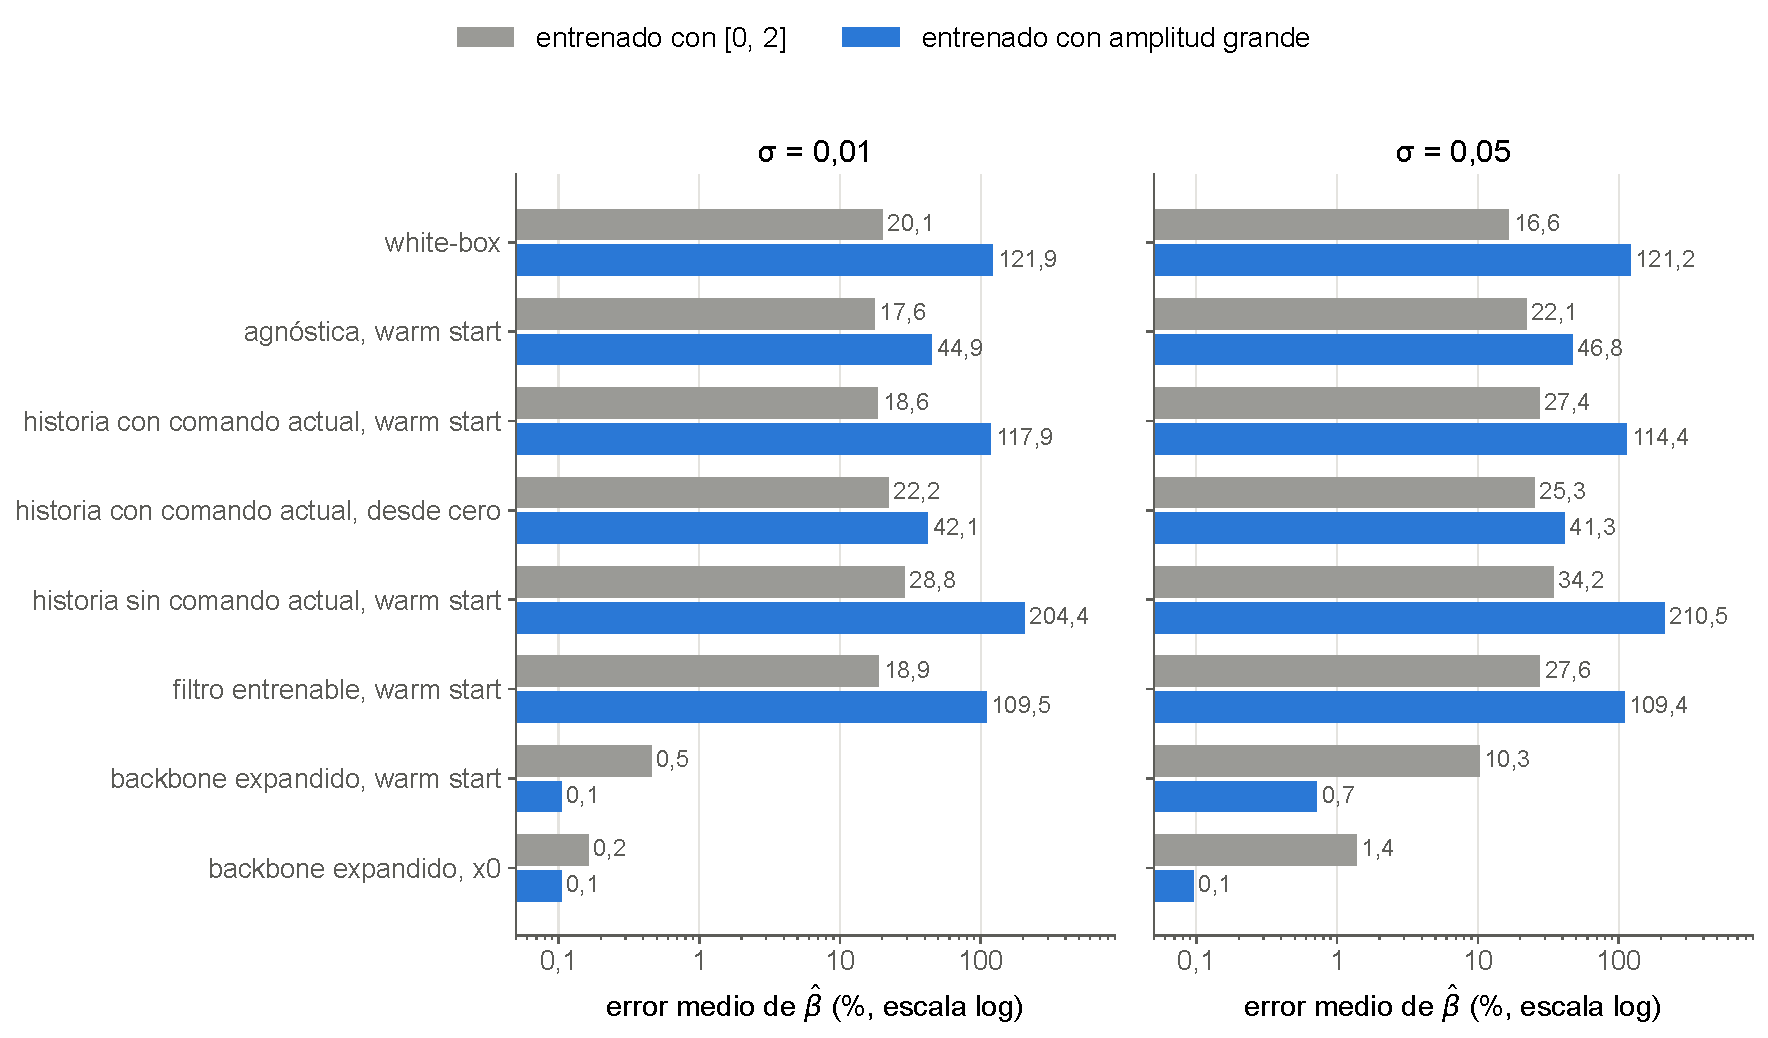
\includegraphics[width=\textwidth]{beta_actuador.pdf}
\caption{Error medio de los diez parámetros del actuador con recorte, entrenando con $[0, 2]$ (gris) y con amplitud grande (azul). Escala logarítmica. Media de tres semillas, con $\sigma = 0{,}01$ (izquierda) y $\sigma = 0{,}05$ (derecha).}
\end{figure}

\section{Lazo cerrado}

Distancia eficaz entre las trayectorias $(E, I)$ del lazo con el modelo y del lazo con el simulador, sobre el último 80~\% de la corrida, con el controlador del paper sin cambios. Mediana de tres semillas, actuador con recorte, $\sigma = 0{,}01$. Entre paréntesis, el mismo modelo entrenado con $[0, 2]$.

\begin{center}
\small
\begin{tabular}{@{}lcccc@{}}
\toprule
actuador con recorte & theta-gamma & gamma 50~ms & theta en rango & gamma en rango \\
\midrule
white-box & 0,037 (0,034) & 0,068 (0,061) & 0,007 (0,001) & 0,021 (0,003) \\
agnóstica & 0,041 (0,034) & 0,071 (0,061) & 0,008 (0,001) & 0,008 (0,003) \\
historia con comando actual & 0,040 (0,049) & 0,075 (0,068) & 0,020 (0,029) & 0,030 (0,044) \\
historia sin comando actual & 0,061 (0,057) & 0,111 (0,076) & 0,072 (0,035) & 0,061 (0,055) \\
filtro entrenable & 0,037 (0,065) & 0,072 (0,067) & 0,004 (0,047) & 0,003 (0,053) \\
backbone expandido & 0,012 (0,035) & 0,008 (0,062) & 0,000 (0,000) & 0,000 (0,000) \\
black-box & 0,033 & 0,064 & 0,002 & 0,004 \\
black-box con historia & 0,036 & 0,078 & 0,003 & 0,004 \\
\bottomrule
\end{tabular}
\end{center}

Con $\sigma = 0{,}05$ los valores cambian menos de 0,01, salvo la historia con comando actual en theta en rango (0,004). El backbone expandido queda en 0,013 en theta-gamma y en gamma, y en 0,012 y 0,008 con x0 entrenable. En la refractaria todos los modelos quedan a 0,007 o menos del lazo con el simulador en las cuatro referencias, con los dos niveles de ruido.

\section{Posibles explicaciones}

Lo que sigue son explicaciones compatibles con lo medido. Las que no tienen una prueba directa llevan al lado la corrida o el análisis que la pondría a prueba.

\hip{El white-box del actuador deforma $\beta$ para imitar la saturación y el filtro.}
Con el recorte activo en un tercio de las muestras, la respuesta del simulador a comandos grandes queda acotada. El white-box no tiene un recorte, y la forma más directa de acotar la respuesta es aplanar la sigmoidea. La dirección de la deformación coincide con eso (media de tres semillas, $\sigma = 0{,}01$). Las pendientes $a_e$ y $a_i$ bajan 36 y 66~\%, y los pesos suben entre 69 y 532~\%, lo que compensa la ganancia perdida en el rango chico. Las constantes de tiempo suben 70 y 51~\%, compatible con imitar el retardo del filtro de 1~ms. Con los datos de $[0, 2]$ el recorte no actuaba y la deformación era de 20~\%.

\hip{El warm start arrastra esa deformación a las correcciones con red.}
Con warm start, las correcciones parten del white-box con 122~\% de error y terminan entre 110 y 204~\%. Desde cero terminan entre 42 y 71~\%. La red se ajusta como corrección alrededor de un $\bh$ ya deformado y el gradiente no lo lleva de vuelta, porque la combinación ya reproduce bien (NRMSE de 1,3 a 1,9). La deformación desde cero tiene otra dirección: en la historia con comando actual, los pesos $w_{IE}$ y $w_{II}$ bajan 66 y 83~\%. Varias combinaciones de $\bh$ y red reproducen igual de bien, y cada arranque cae en una distinta.

\hip{Las redes no reconstruyen el término faltante aunque reproduzcan la salida.}
El R² de las correcciones contra el término faltante queda entre $-0{,}7$ y 0,25, con NRMSE de 1,3 a 1,9. Si la red sola no puede representar filtro más recorte, la deformación de $\beta$ es la única salida; si puede, el problema es de identificabilidad entre $\beta$ y la red. Lo distingue la tanda e28, con $\beta$ fijo en los verdaderos y solo la red entrenable, que ya está preparada. Con los datos de $[0, 2]$ y el actuador con tanh, esa prueba dio R² de 0,84 para la historia con comando actual, 0,74 para el filtro entrenable, 0,19 para la historia sin comando actual y $-0{,}20$ para la agnóstica.

\hip{La historia sin comando actual empeora en lazo cerrado.}
Sin el comando del instante actual, la red no puede reconstruir el estado del filtro, que depende del comando más reciente. El e20 lo mostró con $\beta$ verdadero (R² de 0,19 contra 0,84 con el comando actual). En lazo cerrado el comando cambia en cada paso del controlador, y ese retraso pesa más que en lazo abierto.

\hip{Reproducir en lazo abierto no alcanza para reproducir el lazo cerrado.}
Las correcciones con historia y el filtro entrenable tienen NRMSE de lazo abierto de 1,3 a 1,9, y la black-box con historia de 1,09. Todos quedan a entre 0,036 y 0,111 del lazo con el simulador en theta-gamma y gamma, y las historias oscilan en los tramos de reposo. Una explicación posible es que el controlador los lleva a combinaciones de comando y estado que el entrenamiento no cubre. Se pone a prueba corriendo cada modelo en lazo abierto con el comando registrado del lazo con el simulador: si el error aparece ahí, depende de la región del espacio; si no aparece, depende de la realimentación.

\hip{En la refractaria todo mejora porque el término faltante crece con la actividad.}
El factor $(1 - r x)$ es más grande cuanto mayor es la actividad. Con comandos grandes, el desvío estándar de $E$ en entrenamiento pasa de 0,17 a 0,34, la fracción del tiempo con $E > 0{,}3$ pasa de 11 a 29~\%, y el término faltante crece de 0,013 a 0,036 en $E$ y de 0,002 a 0,014 en $I$. Un término más grande respecto del ruido es más fácil de separar de $\beta$, y eso coincide con que la agnóstica ya no necesite warm start (1,8~\% desde cero, antes 18~\%).

\hip{El sesgo por ruido en las ventanas casi desaparece por la misma razón.}
El sesgo venía del ruido en el estado inicial de cada ventana de 5~ms. Con la respuesta dos a tres veces más grande, el mismo ruido pesa menos. El white-box sobre la planta ideal pasa de 9,8 a 0,63~\% de error de $\bh$ con $\sigma = 0{,}05$, y el x0 entrenable deja de cambiar los resultados salvo en el backbone expandido con $\sigma = 0{,}05$.

\hip{El nivel del recorte se identifica porque ahora recibe gradiente.}
Con comandos de hasta 12, el recorte inicial en 10 actúa en los escenarios de mayor amplitud, recibe gradiente y baja hasta 3. Con comandos menores a 2 nunca actuaba. Inicializar el nivel por debajo de 2, que estaba pendiente, deja de hacer falta con estos datos.

\section{Pendientes}

\begin{itemize}[leftmargin=*,itemsep=0.3em]
\item Correr e28, $\beta$ verdadero fijo y red entrenable sobre los datos de amplitud: agnóstica, las dos historias y el filtro entrenable en el actuador, y la agnóstica en la refractaria, con los dos ruidos y tres semillas (30 corridas).
\item Evaluar las correcciones con red en lazo abierto con el comando registrado del lazo con el simulador.
\item Decidir cómo entran las dos tandas al informe: como dos regímenes de identificación, o la de amplitud en lugar de la de $[0, 2]$.
\end{itemize}

\end{document}
